\section{Resultados}

\begin{table}[h]
\centering

\label{tab:results-summary}
\scriptsize
\setlength{\tabcolsep}{4pt}
\sisetup{table-format=1.3}
\begin{tabularx}{\linewidth}{@{}l X S S S S@{}}
\toprule
\textbf{Classifier} & \textbf{Best parameters} & {\textbf{Train acc}} & {\textbf{5-fold CV accuracy}} \\
\midrule
DecisionTree (baseline) &
\textit{defaults} &
& 0.659\\

DecisionTree (tuned) &
\makecell[tl]{\texttt{criterion=gini, max\_depth=3,}\\
\texttt{min\_samples\_leaf=1, min\_samples\_split=2,}\\
\texttt{max\_features=None, class\_weight=None,}\\
\texttt{splitter=best}} &
0.700  & 0.719\\
\bottomrule
\end{tabularx}
\caption{Resumen de resultados por modelo.}
\end{table}

% --- Figura: matrices de confusión lado a lado ---
\begin{figure}[h]
  \centering
  \begin{subfigure}[t]{0.48\linewidth}
    \centering
    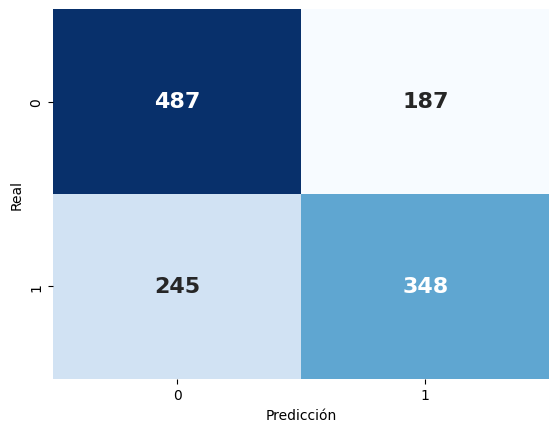
\includegraphics[width=\linewidth]{figures/decision_tree_baseline_cm.png}
    \caption{Baseline (normalizada por fila)}
    \label{fig:cm-base}
  \end{subfigure}\hfill
  \begin{subfigure}[t]{0.48\linewidth}
    \centering
    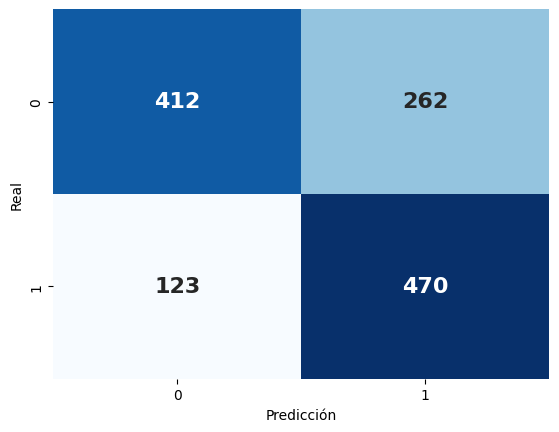
\includegraphics[width=\linewidth]{figures/decision_tree_tunned_cm.png}
    \caption{Tuned (normalizada por fila)}
    \label{fig:cm-tuned}
  \end{subfigure}
  \caption{Comparativa de matrices de confusión. Misma escala (0–1), mismo orden de clases.}
  \label{fig:cm-compare}
\end{figure}


\paragraph{Lectura breve.}
El modelo ajustado (\emph{tuned}) mejora la \textbf{Accuracy} (0.659 $\rightarrow$ 0.700) y el \textbf{F1 (macro)}, con resultados
coherentes con la \textbf{5-fold CV acc} (0.719). En la comparación de matrices se aprecia una reducción de errores
clave respecto al baseline (p.\,ej., menor tasa de falsos negativos en la clase positiva), manteniendo una
distribución de aciertos más equilibrada por clase.